\documentclass[article]{jss}

%% -- LaTeX packages and custom commands ---------------------------------------

%% recommended packages
\usepackage{thumbpdf,lmodern}

%% additional packages
\usepackage{amssymb,amsmath}

%% new custom commands
\newcommand{\class}[1]{`\code{#1}'}
\newcommand{\fct}[1]{\code{#1()}}

%% For Sweave-based articles about R packages:
%% need no \usepackage{Sweave}



%% -- Article metainformation (author, title, ...) -----------------------------

%% - \author{} with primary affiliation
%% - \Plainauthor{} without affiliations
%% - Separate authors by \And or \AND (in \author) or by comma (in \Plainauthor).
%% - \AND starts a new line, \And does not.
\author{Lennart Oelschl\"ager \\Bielefeld University \And Dietmar Bauer\\Bielefeld University}
\Plainauthor{Lennart Oelschl\"ager, Dietmar Bauer}

%% - \title{} in title case
%% - \Plaintitle{} without LaTeX markup (if any)
%% - \Shorttitle{} with LaTeX markup (if any), used as running title
\title{\pkg{RprobitB}: Bayes Estimation of Discrete Choice Behavior Heterogeneity via Probit Models in \proglang{R}}
\Plaintitle{RprobitB: Bayes Estimation of Discrete Choice Behavior Heterogeneity via Probit Models in R}
\Shorttitle{RprobitB}

%% - \Abstract{} almost as usual
\Abstract{
\pkg{RprobitB} is an \proglang{R} package for Bayes estimation of probit models with a special focus on modeling choice behavior heterogeneity. In comparison to competing packages it places a focus on approximating the mixing distribution via a latent mixture of Gaussian distributions and thereby providing a classification of deciders. It provides tools for data management, model estimation via Markov Chain Monte Carlo Simulation, diagnostics tools for the Gibbs sampling and a prediction function. This paper demonstrates the functionalities of \pkg{RprobitB} on known choice datasets and compares estimation results across packages.
}

%% - \Keywords{} with LaTeX markup, at least one required
%% - \Plainkeywords{} without LaTeX markup (if necessary)
%% - Should be comma-separated and in sentence case.
\Keywords{discrete choice, probit models, heterogeneity, Bayes estimation, \proglang{R}}
\Plainkeywords{discrete choice, probit models, heterogeneity, Bayes estimation, R}

%% - \Address{} of at least one author
%% - May contain multiple affiliations for each author
%%   (in extra lines, separated by \emph{and}\\).
%% - May contain multiple authors for the same affiliation
%%   (in the same first line, separated by comma).
\Address{
  Lennart Oelschl\"ager\\
  Department of Business Administration and Economics\\
  Bielefeld University\\
  Postfach 10 01 31\\
  E-mail: \email{lennart.oelschlaeger@uni-bielefeld.de}
}

\begin{document}
%% I have no idea what this does. Maybe we need this in the future.
%% \SweaveOpts{concordance=TRUE}

%% -- Introduction -------------------------------------------------------------

%% - In principle "as usual".
%% - But should typically have some discussion of both _software_ and _methods_.
%% - Use \proglang{}, \pkg{}, \fct{} and \code{} markup throughout the manuscript.
%% - If such markup is in (sub)section titles, a plain text version has to be
%%   added as well.
%% - All software mentioned should be properly \cite-d.
%% - All abbreviations should be introduced.
%% - Unless the expansions of abbreviations are proper names (like "Journal
%%   of Statistical Software" above) they should be in sentence case (like
%%   "generalized linear models" below).

\section{Introduction}
\label{sec:intro}

%% Short introduction
The multinomial probit model is one of the most widely-used statistical models to explain the choices that individuals make among a discrete set of alternatives, which is of central interest in many scientific areas, for example in transportation and marketing. In many such choice scenarios it is reasonable to assume, that the preferences of the decision makers are non-homogeneous. Based on personal characteristics, deciders generally weight attributes like time and cost differently. Heterogeneity in choice behavior can be modeled using mixing distributions for the coefficients. Recently, Oelschlaeger and Bauer proposed a new instrument for approximating the underlying mixing distribution that combines Bayes estimation and semi-parametric methods. This paper presents the implementation of the methodology in the \proglang{R} package \pkg{RprobitB}.

%% Overview RUMs
Traditionally, discrete choice models are interpreted as random utility models, including the multinomial logit (MNL) and the multinomial probit (MNP) model as the most prominent members. The MNL model affords straightforward analysis but suffers from the well-known independence of irrelevant alternatives assumption. In contrast, the MNP model avoids this assumption, which however comes at the price of more complex parameter estimation, cf. \cite{Train:09}. In their basic form, these models often fail to take into account heterogeneity of individual deciders, cf. \cite{Train:09}, Chapter 6, or \cite{Train:16}. A concrete example of heterogeneous preferences is constituted by the value of travel time, cf. \cite{Cirillo:06}. Modeling heterogeneity in preferences is indispensable in such cases and has been elaborated in both the MNL and the MNP model by imposing mixing distributions on the coefficients, cf. \cite{Train:09} and \cite{Bhat:11}.

%How are the mixing distribution specified currently?
Specifying these mixing distributions is an important part of the model selection. In absence of alternatives, it has been common practice so far to try different types of standard parametric distributions (including the normal, log-normal, uniform and tent distribution) and to perform a likelihood value-based model selection, cf. \cite{Train:09}, Chapter 6. Aiming to capture correlation patterns across parameters, \cite{Fountas:18} and \cite{Fountas:19} apply multivariate normal mixing distributions in their probit models, which however comes at the price of imposing the rather strong normality assumption on their parameters.

In order to alleviate these restrictions \cite{Train:16} proposes a non-parametric approach based on grid methods. Building on the ideas of \cite{Train:16} and \cite{Bhat:18} recently \cite{Bauer:19} introduced procedures for non-parametrically estimating latent class mixed multinomial probit models where the number of classes is chosen iteratively in the algorithm. These procedures have been demonstrated to be useful in reasonable sized cross-sectional data sets. However, for large panel data sets with a significant number of choice occasions per person, the approach is numerically extremely demanding in particular due to its non-parametric nature and has to deal with the curse of dimensionality.

%What is the potential benefit of Bayesian estimation?
In the Bayesian framework \cite{Scaccia:10} presents the idea to estimate latent class logit models with a fixed prespecified number of Gaussian components. This approach does not require the maximization of the likelihood while at the same time it allows for approximation of the underlying mixing distribution. The same idea has also been applied to probit models, cf. \cite{Xiong:13} for an analysis of adolescent driver-injury data. In both cases however, the specification of the number of latent classes is based only on a trial-and-error strategy.

%What approach do we suggest to specify the mixing distributions?
Oelschlaeger and Bauer presents a more flexible approach that combines the ideas of a Bayesian framework, approximating the mixing distribution through a mixture of normal distributions and updates on the number of latent classes within the algorithm analogously to \cite{Bauer:19}. As a consequence, the procedure unites the benefits of a reduced numerical complexity for the estimation compared to the non-parametric likelihood maximization approach and the ability to approximate any mixing distribution. Presenting simulation results on artificial test cases, it is shown that the approach is capable of approximating the underlying mixing distributions and thereby guiding the specification of mixing distributions for real-world applications.

%% Comparison to other packages
This packages adds to the line of discrete choice software packages in R in the following way: Its focus is entirely on Bayesian estimation, thereby it differs from the packages Rchoice. Furthermore, it places a focus on modeling choice behaviour heterogeneity by approximating the underlying mixing distribution through a latent mixture of normal distributions. The method is explained in detail in Oelschlaeger and Bauer.

%% Article overview
In this article we present the methodology, give an overview over the functionality of the package and apply the package to datasets. Some of them were already analysed and we aim to reconstruct their findings. In addition, we added two datasets that are especially appropriate for the RprobitB package in modeling choice behaviour heterogeneits. The first one is a dataset of contraception choice from the German family panel pairfam. It contains repeated observations of males and femals over several years having different social demographics and relationship status choosing different means of contraception. This choice a priori can be considered to be very hetereogenous and dependent on factors not directly observable by the researcher. The second application deals with the opening choice of chess players depending on their and their openents playing strenght measured in the popular measure system Elo, their gender and nationality. Like the contraception example, this choice a priori can be considers to depend on psychological factors that are not directly observable by the researcher. By applying the functionality of this package we demonstrate how we are able to classify the players into different categories of playing style.

%% -- Manuscript ---------------------------------------------------------------

%% - In principle "as usual" again.
%% - When using equations (e.g., {equation}, {eqnarray}, {align}, etc.
%%   avoid empty lines before and after the equation (which would signal a new
%%   paragraph.
%% - When describing longer chunks of code that are _not_ meant for execution
%%   (e.g., a function synopsis or list of arguments), the environment {Code}
%%   is recommended. Alternatively, a plain {verbatim} can also be used.
%%   (For executed code see the next section.)
%% - Tables are placed at the top of the page
%%   (\verb|[t!]|), centered (\verb|\centering|), with a caption below the table,
%%   column headers and captions in sentence style, and if possible avoiding
%%   vertical lines.

\section{The method} \label{sec:method}

Content.

\subsection{The mixed multinomial probit model} \label{subsec:mnp}


Assume that we observe the choices of $N$ decision makers which decide between $J$ alternatives at each of $T$ choice occasions.\footnote{For notational simplicity, we use a balanced panel where the number of choice occasions $T$ is assumed to be the same for each decision maker. Differences however are straightforward to implement.} Specific to each decision maker, alternative and choice occasion, we furthermore observe $P_f+P_r$ choice attributes that we use to explain the choices. The first $P_f$ attributes are connected to fixed coefficients, the other $P_r$ attributes to random coefficients following a joint  distribution mixed across decision makers. Person $n$'s utility $\tilde{U}_{ntj}$ for alternative $j$ at choice occasion $t$ is modelled as
\begin{equation}
\tilde{U}_{ntj} = \tilde{W}_{ntj}'\alpha + \tilde{X}_{ntj}'\beta_n + \tilde{\epsilon}_{ntj}
\end{equation}
for $n=1,\dots,N$, $t=1,\dots,T$ and $j=1,\dots,J$, where
\begin{itemize}
	\item $\tilde{W}_{ntj}$ is a vector of $P_f$ characteristics of $j$ as faced by  $n$ at $t$ corresponding to the fixed coefficient vector $\alpha \in {\mathbb R}^{P_f}$,
	\item $\tilde{X}_{ntj}$ is a vector of $P_r$ characteristics of $j$ as faced by  $n$ at $t$ corresponding to the random, decision maker-specific coefficient vector $\beta_n \in {\mathbb R}^{P_r}$, where $\beta_n$ is distributed according to some $P_r$-variate distribution $g_{P_r}$,
	\item and $(\tilde{\epsilon}_{nt:}) = (\tilde{\epsilon}_{nt1},\dots,\tilde{\epsilon}_{ntJ})' \sim \text{MVN}_J (0,\tilde{\Sigma})$ is the models' error term vector for $n$ at $t$, which in the probit model is assumed to be multivariate normally distributed with zero mean and covariance matrix $\tilde{\Sigma}$.
\end{itemize}
As is well known, any utility model needs to be normalized with respect to level and scale in order to be identified, cf. \cite{Train:09}, Section 5.2. Therefore, we consider the transformed model
\begin{equation}
\label{eq:model}
U_{ntj} = W_{ntj}'\alpha + X_{ntj}'\beta_n + \epsilon_{ntj},
\end{equation}
$n=1,\dots,N$, $t=1,\dots,T$ and $j=1,\dots,J-1$, where (choosing $J$ as the reference alternative) $U_{ntj}=\tilde{U}_{ntj} - \tilde{U}_{ntJ}$, $W_{ntj}=\tilde{W}_{ntj}-\tilde{W}_{ntJ}$, $X_{ntj}=\tilde{X}_{ntj}-\tilde{X}_{ntJ}$ and $\epsilon_{ntj}=\tilde{\epsilon}_{ntj}-\tilde{\epsilon}_{ntJ}$, where $(\epsilon_{nt:}) = (\epsilon_{nt1},...,\epsilon_{nt(J-1)})'  \sim \text{MVN}_{J-1} (0,\Sigma)$ and $\Sigma$ denotes a covariance matrix with the top-left element restricted to one. \cite{Train:09} provides an algorithm on how to transform $\tilde{\Sigma}$ to $\Sigma$. While taking utility differences in order to normalize the model with respect to level is a standard procedure, alternatives to fixing an error term variance in order to normalize with respect to scale exist, cf. \cite{Mori:14}.

Let $y_{nt}=j$ denote the event that decision maker $n$ chooses alternative $j$ at choice occasion~$t$. Assuming utility maximizing behaviour of the decision makers, the decisions are linked to the utilities via
%($U_{ntJ}=0$)
%$$
%y_{nt}=j \Leftrightarrow U_{ntj} = \max_{1 \le i \le J} U_{nti}, j=1,...,J.
%$$
%
\begin{equation}
\label{eq:choice}
y_{nt} = \sum_{j=1}^{J-1} j\cdot 1 \left (U_{ntj}=\max_i U_{nti}>0 \right) + J \cdot 1\left (U_{ntj}<0 ~\text{for all}~j\right),
\end{equation}
where $1(A)$ equals $1$ if condition $A$ is true and $0$ else.


\subsection{Approximating the mixing distribution} \label{subsec:amd}

We approximate the mixing distribution $g_{P_r}$ for the random coefficients\footnote{Here and below we use the abbreviation $(\beta_n)_n$ as a shortcut to $(\beta_n)_{n =1,...,N}$ the collection of vectors $\beta_n,n=1,...,N$.} $\beta=(\beta_n)_{n}$ by a mixture of $P_r$-variate normal densities $\phi_{P_r}$ with mean vectors $b=(b_c)_{c}$ and covariance matrices $\Omega=(\Omega_c)_{c}$ using $C$ components, i.e.
\begin{equation}
\label{eq:mixture}
\beta_n\mid b,\Omega \sim \sum_{c=1}^{C} s_c \phi_{P_r} (\cdot \mid b_c,\Omega_c),
\end{equation}
where $(s_c)_{c}$ are weights satisfying $0 < s_c\leq 1$ for $c=1,\dots,C$ and $\sum_c s_c=1$.
One interpretation of the latent class model is obtained by introducing variables $z=(z_n)_n$ allocating each decision maker $n$ to class $c$ with probability $s_c$, i.e.
\begin{equation}
\label{eq:mixture_allocation}
\Prob(z_n=c)=s_c \quad \text{and} \quad \beta_n \mid z,b,\Omega \sim \phi_{P_r}(\cdot \mid b_{z_n},\Omega_{z_n}).
\end{equation}
The model defined by equations \eqref{eq:model}, \eqref{eq:choice} and \eqref{eq:mixture_allocation} is what we call the latent class mixed multinomial probit model. We note that the model collapses to the (normally) mixed multinomial probit model if $P_r>0$ and $C=1$ and to the basic MNP model if $P_r=0$.


\subsection{The Bayesian framework} \label{subsec:bayes}

Our Bayesian analysis of the latent class mixed multinomial probit model builds upon the Bayesian framework of the MNP model, which has been developed by \cite{McCulloch:94}, \cite{Nobile:98}, \cite{Allenby:98}, and \cite{Imai:05}. Their work provides Markov chain Monte Carlo algorithms for numerically computing Bayes estimates of the posterior distribution of the MNP model parameters. A key ingredient is the concept of data augmentation, cf. \cite{Albert:93}, which treats the latent utilities as parameters themselves. Conditional on the latent utilities, the MNP model constitutes a standard Bayesian linear regression set-up, which renders drawing from the posterior distribution feasible without the need to evaluate any likelihood.

This section defines the Bayesian framework that we use in order to estimate the latent class mixed multinomial probit model. Next outlines the choice of prior distributions. We apply an eight-component Gibbs sampler to approximate the models' joint posterior distribution. The number of latent classes is updated within the Gibbs sampler.

Bayesian analysis enables to impose prior beliefs on the model parameters. It is possible to either express strong a priori knowledge using informative prior distributions or to express vague knowledge using diffuse prior distributions. For our model, we apply the following conjugate priors:
\begin{itemize}
	\item $(s_1,\dots,s_C)\sim D_C(\delta)$, where $D_C(\delta)$ denotes the $C$-dimensional Dirichlet distribution with concentration parameter vector $\delta = (\delta_1,\dots,\delta_C)$,
	\item $\alpha\sim \text{MVN}_{P_f}(\psi,\Psi)$,
	\item $b_c \sim \text{MVN}_{P_r}(\xi,\Xi)$, independent for all $c$,
	\item $\Omega_c \sim W^{-1}_{P_r}(\nu,\Theta)$, independent for all $c$, where $W^{-1}_{P_r}(\nu,\Theta)$ denotes the $P_r$-dimensional inverse Wishart distribution with $\nu$ degrees of freedom and scale matrix $\Theta$,
	\item and $\Sigma \sim W^{-1}_{J-1}(\kappa,\Lambda)$.
\end{itemize}

The parameters of the prior distributions can be chosen based on estimation results of similar choice settings, resulting in informative priors. We found that priors do not have large impact on results. Because we need much data. We applied the diffuse prior approach, setting $\delta_1=\dots=\delta_C=1$; $\psi$ and $\xi$ equal to the zero vector; $\Psi$ and $\Xi$ equal to the identity matrix with value 10 on the diagonal; $\nu$ and $\kappa$ equal to $P_r+2$ and $J+1$, respectively (to obtain proper priors); $\Theta$ and $\Lambda$ equal to the identity matrix.

Sampling from the joint posterior distribution in the Gibbs sampler proceeds by iteratively drawing and updating each model parameter conditional on the other parameters.

\paragraph{Updating $s$.} The class weights are drawn from the Dirichlet distribution
\begin{equation}
(s_1,\dots,s_C)\mid \delta,z \sim D_C(\delta_1+m_1,\dots,\delta_C+m_C),
\end{equation}
where for $c=1,\dots,C$, $m_c=\#\{n:z_n=c\}$ denotes the current absolute class size. Mind that the model is invariant to permutations of the class labels $1,\dots,C$. For that reason, we accept an update only if the ordering $s_1<\dots<s_C$ holds, thereby ensuring a unique labelling of the classes.

\paragraph{Updating $z$.} Independently for all $n$, we update the allocation variables $(z_n)_n$ from their conditional distribution
\begin{equation}
\Prob(z_n=c\mid s,\beta,b,\Omega )=\frac{s_c\phi_{P_r}(\beta_n\mid b_c,\Omega_c)}{\sum_c s_c\phi_{P_r}(\beta_n\mid b_c,\Omega_c)}.
\end{equation}

\paragraph{Updating $b$.} The class means $(b_c)_c$ are updated independently for all $c$ via
\begin{equation}
b_c\mid \Xi,\Omega,\xi,z,\beta \sim\text{MVN}_{P_r}\left( \mu_{b_c}, \Sigma_{b_c}  \right),
\end{equation}
where $\mu_{b_c}=(\Xi^{-1}+m_c\Omega_c^{-1})^{-1}(\Xi^{-1}\xi +m_c\Omega_c^{-1}\bar{b}_c)$, $\Sigma_{b_c}=(\Xi^{-1}+m_c\Omega_c^{-1})^{-1}$, $\bar{b}_c=m_c^{-1}\sum_{n:z_n=c} \beta_n$.

\paragraph{Updating $\Omega$.} The class covariance matrices $(\Omega_c)_c$ are updated independently for all $c$ via
\begin{equation}
\Omega_c \mid \nu,\Theta,z,\beta,b \sim W^{-1}_{P_r}(\mu_{\Omega_c},\Sigma_{\Omega_c}),
\end{equation}
where $\mu_{\Omega_c}=\nu+m_c$ and $\Sigma_{\Omega_c}=\Theta^{-1} + \sum_{n:z_n=c} (\beta_n-b_c)(\beta_n-b_c)'$.

\paragraph{Updating $U$.} Independently for all $n$ and $t$ and conditionally on the other components, the utility vectors $(U_{nt:})$ follow a $J-1$-dimensional truncated multivariate normal distribution, where the truncation points are determined by the choices $y_{nt}$. To sample from a truncated multivariate normal distribution, we apply a sub-Gibbs sampler, following the approach of \cite{Geweke:98}:
\begin{equation}
U_{ntj} \mid U_{nt(-j)},y_{nt},\Sigma,W,\alpha,X,\beta
\sim \mathcal{N}(\mu_{U_{ntj}},\Sigma_{U_{ntj}}) \cdot \begin{cases}
1(U_{ntj}>\max(U_{nt(-j)},0) ) & \text{if}~ y_{nt}=j\\
1(U_{ntj}<\max(U_{nt(-j)},0) ) & \text{if}~ y_{nt}\neq j
\end{cases},
\end{equation}
where $U_{nt(-j)}$ denotes the vector $(U_{nt:})$ without the element $U_{ntj}$, $\mathcal{N}$ denotes the univariate normal distribution, $\Sigma_{U_{ntj}} = 1/(\Sigma^{-1})_{jj}$ and
\begin{equation}
\mu_{U_{ntj}} = W_{ntj}'\alpha + X_{ntj}'\beta_n - \Sigma_{U_{ntj}} (\Sigma^{-1})_{j(-j)}   (U_{nt(-j)} - W_{nt(-j)}'\alpha - X_{nt(-j)}' \beta_n ),
\end{equation}
where $(\Sigma^{-1})_{jj}$ denotes the $(j,j)$th element of $\Sigma^{-1}$, $(\Sigma^{-1})_{j(-j)}$ the $j$th row without the $j$th entry, $W_{nt(-j)}$ and $X_{nt(-j)}$ the coefficient matrices $W_{nt}$ and $X_{nt}$, respectively, without the $j$th column.

\paragraph{Updating $\alpha$.} Updating the fixed coefficient vector $\alpha$ is achieved by applying the formula for Bayesian linear regression of the regressors $W_{nt}$ on the regressands $(U_{nt:})-X_{nt}'\beta_n$, i.e.
\begin{equation}
\alpha \mid \Psi,\psi,W,\Sigma,U,X,\beta \sim \text{MVN}_{P_f}(\mu_\alpha,\Sigma_\alpha),
\end{equation}
where $\mu_\alpha = \Sigma_\alpha (\Psi^{-1}\psi + \sum_{n=1,t=1}^{N,T} W_{nt} \Sigma^{-1} ((U_{nt:})-X_{nt}'\beta_n) )$ and $\Sigma_\alpha = (\Psi^{-1} + \sum_{n=1,t=1}^{N,T} W_{nt}\Sigma^{-1} W_{nt}^{'} )^{-1}$.

\paragraph{Updating $\beta$.} Analogously to $\alpha$, the random coefficients $(\beta_n)_n$ are updated independently via
\begin{equation}
\beta_n \mid \Omega,b,X,\Sigma,U,W,\alpha \sim \text{MVN}_{P_r}(\mu_{\beta_n},\Sigma_{\beta_n}),
\end{equation}
where $\mu_{\beta_n} = \Sigma_{\beta_n} (\Omega_{z_n}^{-1}b_{z_n} + \sum_{t=1}^{T} X_{nt} \Sigma^{-1} (U_{nt}-W_{nt}'\alpha) )$ and $\Sigma_{\beta_n} = (\Omega_{z_n}^{-1} + \sum_{t=1}^{T} X_{nt}\Sigma^{-1} X_{nt}^{'} )^{-1}$ .

\paragraph{Updating $\Sigma$.}
The error term covariance matrix $\Sigma$ is updated by means of
\begin{equation}
\Sigma \mid \kappa,\Lambda,U,W,\alpha,X,\beta \sim W^{-1}_{J-1}(\kappa+NT,\Lambda+S), \\
\end{equation}
where $S = \sum_{n=1,t=1}^{N,T} \epsilon_{nt} \epsilon_{nt}'$ and $\epsilon_{nt} = (U_{nt:}) - W_{nt}'\alpha - X_{nt}'\beta_n$.

\vspace{0.5cm}
Since $\Sigma$ is drawn from the unrestricted space of symmetric, positive-definite matrices, the samples still lack identification. Therefore, subsequent to the sampling, the normalizations $\alpha^{(i)}/\sqrt{(\Sigma^{(i)})_{11}}$, $b_c^{(i)}/\sqrt{(\Sigma^{(i)})_{11}}$, $\Omega_c^{(i)}/(\Sigma^{(i)})_{11}$, $c=1,\dots,C$ and $\Sigma^{(i)}/(\Sigma^{(i)})_{11}$ are required for the $i$th updates in each iterations $i$, cf. \cite{Imai:05}, where $(\Sigma^{(i)})_{11}$ denotes the top-left element of $\Sigma^{(i)}$. The draws for $s$ do not need to be normalized. The remaining parameters could be normalized, if the results are of interest in the analysis.

%Potential to be shortened
The theory behind Gibbs sampling constitutes that the sequence of samples produced by the updating scheme can be considered as a Markov chain with stationary distribution equal to the desired joint posterior distribution. It takes a certain number of iterations for that stationary distribution to be approximated reasonably well. Therefore, it is common practise to discard the first $B$ out of $R$ samples (the so-called burn-in period). Furthermore, correlation between nearby samples should be expected. In order to obtain independent samples, we consider only every $Q$th sample when averaging values to compute parameter statistics like expectation and standard deviation. Adequate values for $R$, $B$ and $Q$ depend on the complexity of the considered Bayesian framework. Per default, we performed $R=100.000$ iterations, discarded the first $B=R/2$ samples and thinned the sequence by keeping every $Q=200$th sample, resulting in a size of $(R-B)/Q=250$ samples for each parameter. The independence of the samples can be verified by computing the serial correlation. The convergence of the Gibbs sampler can be checked by considering trace plots and comparing the estimates for different sizes of the burn-in period.

Updating the number $C$ of latent classes is done within the Gibbs sampler by executing the following weight-based updating scheme.
\begin{itemize}
	\item We remove class $c$, if $s_c<\epsilon_{\text{min}}$, i.e. if the class weight $s_c$ drops below some threshold $\epsilon_{\text{min}}$. This case indicates that class $c$ has a negligible impact on the mixing distribution.
	\item We split class $c$ into two classes $c_1$ and $c_2$, if $s_c>\epsilon_\text{max}$. This case indicates that class $c$ has a high influence on the mixing distribution whose approximation can potentially be improved by increasing the resolution in directions of high variance. Therefore, the class means $b_{c_1}$ and $b_{c_2}$ of the new classes $c_1$ and $c_2$ are shifted in opposite directions from the class mean $b_c$ of the old class $c$ in the direction of the highest variance.
	\item We join two classes $c_1$ and $c_2$ to one class $c$, if $\lVert b_{c_1} - b_{c_2} \rVert<\epsilon_{\text{distmin}}$, i.e. if the euclidean distance between the class means $b_{c_1}$ and $b_{c_2}$  drops below some threshold $\epsilon_{\text{distmin}}$. This case indicates location redundancy which should be repealed. The parameters of $c$ are assigned by adding the values of $s$ from $c_1$ and $c_2$ and averaging the values for $b$ and $\Omega$.
\end{itemize}
These rules contain choices on the values for $\epsilon_{\text{min}}$, $\epsilon_{\text{max}}$ and $\epsilon_{\text{distmin}}$. Per default, we set $\epsilon_{\text{min}}=0.01$ and $\epsilon_{\text{max}}=0.7$. The adequate value for $\epsilon_{\text{distmin}}$ depends on the scale of the parameters. In our case, we set $\epsilon_{\text{distmin}}=0.1$. We performed the strategy to start with a high number of 10 latent classes and executing the updating scheme discussed above within the second half of the burn-in period. The scheme is executed only every 50th iteration to allow for readjustments after each update.


\subsection{Predictions} \label{subsec:pred}


\section{Package overview} \label{sec:overview}

\pkg{RprobitB} can be installed from CRAN via the \code{install.packages("RprobitB")} command. After installation, the package is loaded by typing:

%
\begin{Schunk}
\begin{Sinput}
> library(RprobitB)
\end{Sinput}
\end{Schunk}
%

Figure \ref{fig:overview} shows a flowchart of the user-level functions. Visibly the functionality can be separated into three groups: Functions for data management, model fitting and model evaluation. Each of these groups is introduced below. The functions are applied in Section \ref{sec:illustrations}.

\begin{figure}
  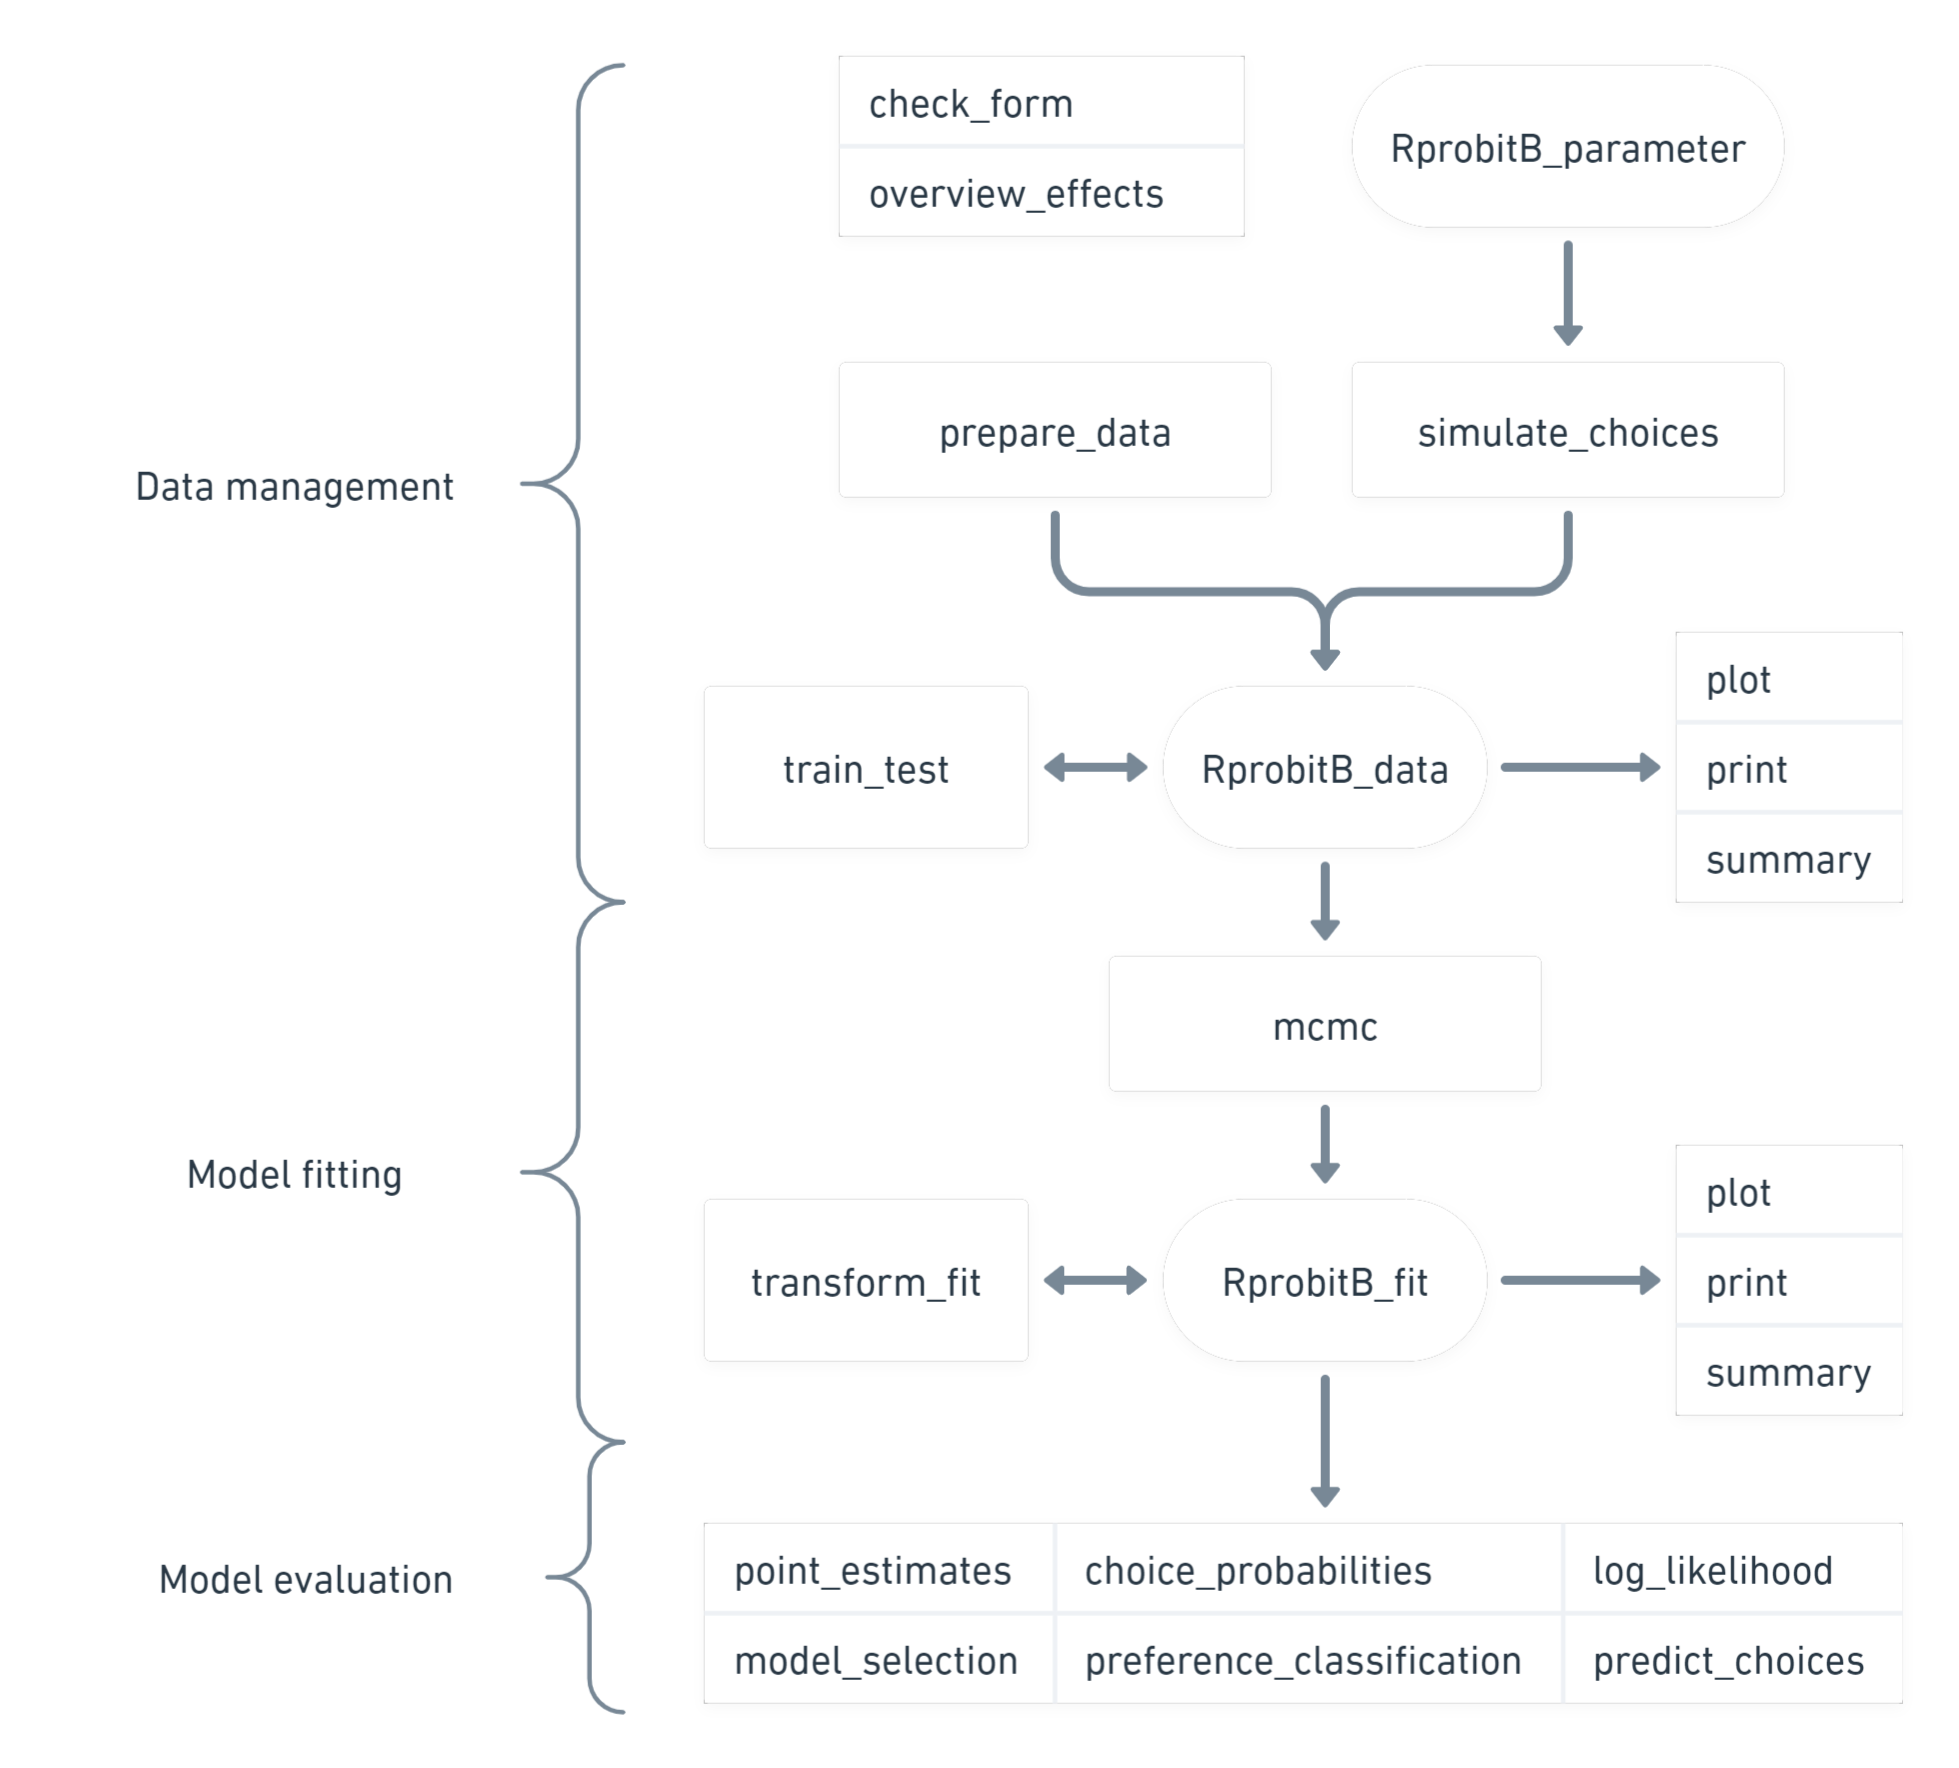
\includegraphics{overview.png}
  \caption{A flowchart of the \pkg{Rprobitb} package. Functions are in rectangle boxes, objects are in circles.}
  \label{fig:overview}
\end{figure}

\subsection{Data mangement} \label{subsec:datamanagement}

The function \fct{prepare\_data} prepares empirical choice data for estimation whereas \fct{simulate\_choices} can simulate choices from a probit model. Both functions create an object of class \class{RprobitB\_data} that can be passed to the estimation function \fct{mcmc} explaind in the next section. Additionally, the \class{RprobitB\_data} object has the three methods \fct{plot}, \fct{print} and \fct{summary} that return data descriptions. Furthermore, the \class{RprobitB\_data} object can be passed to the \fct{train\_test} function that splits the dataset into a train and a test subsample for model validation.

The \fct{prepare\_data} takes the following inputs:
%
\begin{Schunk}
\begin{Sinput}
> args(prepare_data)
\end{Sinput}
\begin{Soutput}
function (form, choice_data, re = NULL, alternatives = NULL, 
    id = "id", idc = NULL, standardize = NULL) 
NULL
\end{Soutput}
\end{Schunk}
%


\subsection{Model fitting} \label{subsec:modelfitting}

\subsection{Model evaluation} \label{subsec:modelevaluation}



%% -- Illustrations ------------------------------------------------------------

%% - Virtually all JSS manuscripts list source code along with the generated
%%   output. The style files provide dedicated environments for this.
%% - In R, the environments {Sinput} and {Soutput} - as produced by Sweave() or
%%   or knitr using the render_sweave() hook - are used (without the need to
%%   load Sweave.sty).
%% - Equivalently, {CodeInput} and {CodeOutput} can be used.
%% - The code input should use "the usual" command prompt in the respective
%%   software system.
%% - For R code, the prompt "R> " should be used with "+  " as the
%%   continuation prompt.
%% - Comments within the code chunks should be avoided - these should be made
%%   within the regular LaTeX text.
%% - Please make sure that all code is properly spaced, e.g., using
%%   \code{y = a + b * x} and \emph{not} \code{y=a+b*x}.
%% - JSS prefers when the second line of code is indented by two spaces.

\section{Illustrations} \label{sec:illustrations}



\subsection{Train dataset} \label{subsec:train}


%
\begin{Schunk}
\begin{Sinput}
> data("Train", package = "mlogit")
> Train$price_A = Train$price_A / 100 * 2.2
> Train$price_B = Train$price_B / 100 * 2.2
\end{Sinput}
\end{Schunk}
%

%
\begin{Schunk}
\begin{Sinput}
> form = choice ~ price | 1 | time + comfort + change
> data = prepare_data(form = form, choice_data = Train)
\end{Sinput}
\end{Schunk}
%

%
\begin{Schunk}
\begin{Sinput}
> m1 = RprobitB::mcmc(data)
\end{Sinput}
\begin{Soutput}
Iteration Info                   ETA (min)
        0 started Gibbs sampling          
     1000                                1
     2000                                1
     3000                                1
     4000                                1
     5000                                1
     6000                                1
     7000                                1
     8000                                1
     9000                                1
    10000 done, total time: 1 min
\end{Soutput}
\end{Schunk}
%

\subsection{Choice of contraception} \label{subsec:contraception}



\subsection{Chess opening} \label{subsec:chess}

%
\begin{Schunk}
\begin{Sinput}
> x = 1
\end{Sinput}
\end{Schunk}
%


%% -- Summary/conclusions/discussion -------------------------------------------

\section{Summary and discussion} \label{sec:summary}

%% The problem
This paper addressed the problem of specifying mixing distributions in the multinomial probit model with a panel data setting, constituting an important part of the model selection for which the literature does not provide much guidance so far. In the absence of alternatives, many applications of the mixed multinomial probit model rely on different types of standard parametric distributions for modelling heterogeneity in preferences in combination with a likelihood-value based model selection. This course of action is very restrictive and imposes strong assumptions on the distribution of the model parameters that could potentially lead to misspecification and biased estimates.

%% Our solution
We proposed a new approach that improves the current specification strategies in several ways: First, our approach does not require any distributional assumption, since the latent class setting is flexible enough to approximate practically any distribution shape and allowing for any correlation pattern. Second, the weight-based updating scheme ensures that the number of latent classes does not need to be prespecified. Third, the imposed Bayesian estimation framework avoids many numerical problems that occur in the frequentist approach. Most notably, no likelihood function has to be evaluated nor approximated. Comparing the numerical estimation speed to the non-parametric frequentist approach of \cite{Bauer:19}, we found that our implementation of the Bayesian approach is at least 10 times faster. The improvement becomes more distinct for panel data settings with a high number of choice occasions. This is due to the fact that for given total sample size $NT$ a large $T$ is beneficial for the Bayesian approach as then the number of vectors $\beta_n,~ n = 1,...,N$ is comparatively small, while in the frequentist approach calculating the likelihood becomes more challenging for increasing the number $T$ of choice situations faced by each of the $N$ individuals. On the other hand, the grid based frequentist approach of \cite{Bauer:19} can potentially achieve a better approximation (especially of point masses) due to the relatively high number of latent classes. However, this approach requires that a suitable grid is set prior to the estimation with a specification of upper bounds for the coefficients. Additionally, the curse of dimensionality plays a crucial role, which is less of a burden in the Bayesian approach. Note that for a fully specified parametric structure these concerns do not play such a big role also for the frequentist approach.

%% Planned extensions
Our simulation results verified that the proposed approach achieves good approximations of the mixing distribution in common choice modelling situations, where the underlying heterogeneity cannot be captured by standard parametric distributions. It would be interesting to apply the approach also to empirical data in the future. Additionally,
further research on how to properly address sign-restricted coefficients is required.

%% -- Optional special unnumbered sections -------------------------------------

\section*{Computational details}

The results in this paper were obtained using
\proglang{R}~4.1.2 with the
\pkg{RprobitB}~1.0.0.9000 package. \proglang{R} itself
and all packages used are available from the Comprehensive
\proglang{R} Archive Network (CRAN) at \url{https://CRAN.R-project.org/}.


\section*{Acknowledgments}

This work has been financed partly by the Deutsche Forschungsgemeinschaft (DFG, German Research Foundation) - Projektnummer 356500581 which is gratefully acknowledged.

%% -- Bibliography -------------------------------------------------------------
%% - References need to be provided in a .bib BibTeX database.
%% - All references should be made with \cite, \citet, \citep, \citealp etc.
%%   (and never hard-coded). See the FAQ for details.
%% - JSS-specific markup (\proglang, \pkg, \code) should be used in the .bib.
%% - Titles in the .bib should be in title case.
%% - Journal titles should not be abbreviated and in title case.
%% - DOIs should be included where available.
%% - Software should be properly cited as well.

\bibliography{refs}


% % %% -- Appendix (if any) --------------------------------------------------------
% % %% - After the bibliography with page break.
% % %% - With proper section titles and _not_ just "Appendix".
% %
% % \newpage
% %
% % \begin{appendix}
% %
% % \section{Installation} \label{app:installation}
% %
% % \end{appendix}
%
% %% -----------------------------------------------------------------------------


\end{document}
